% This file was created with tikzplotlib v0.9.17.
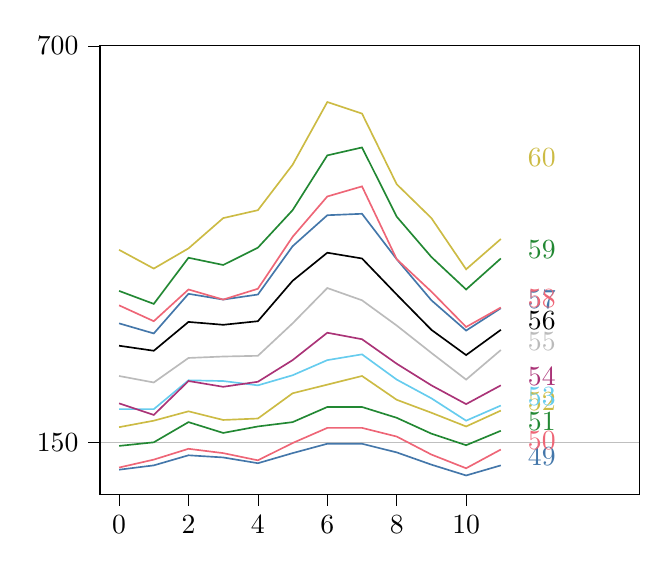
\begin{tikzpicture}

\definecolor{color0}{rgb}{0.266666666666667,0.466666666666667,0.666666666666667}
\definecolor{color1}{rgb}{0.933333333333333,0.4,0.466666666666667}
\definecolor{color2}{rgb}{0.133333333333333,0.533333333333333,0.2}
\definecolor{color3}{rgb}{0.8,0.733333333333333,0.266666666666667}
\definecolor{color4}{rgb}{0.4,0.8,0.933333333333333}
\definecolor{color5}{rgb}{0.666666666666667,0.2,0.466666666666667}

\begin{axis}[
tick align=outside,
tick pos=left,
x grid style={white!69.0196078431373!black},
xmin=-0.55, xmax=15,
xtick style={color=black},
xtick={0,2,4,6,8,10},
xticklabels={
  \(\displaystyle 0\),
  \(\displaystyle 2\),
  \(\displaystyle 4\),
  \(\displaystyle 6\),
  \(\displaystyle 8\),
  \(\displaystyle 10\)
},
ymajorgrids,
ymin=78.1, ymax=700,
ytick style={color=black},
ytick={150,700},
yticklabels={\(\displaystyle 150\),\(\displaystyle 700\)}
]
\addplot [semithick, color0]
table {%
0 112
1 118
2 132
3 129
4 121
5 135
6 148
7 148
8 136
9 119
10 104
11 118
};
\addplot [semithick, color1]
table {%
0 115
1 126
2 141
3 135
4 125
5 149
6 170
7 170
8 158
9 133
10 114
11 140
};
\addplot [semithick, color2]
table {%
0 145
1 150
2 178
3 163
4 172
5 178
6 199
7 199
8 184
9 162
10 146
11 166
};
\addplot [semithick, color3]
table {%
0 171
1 180
2 193
3 181
4 183
5 218
7 242
8 209
9 191
10 172
11 194
};
\addplot [semithick, color4]
table {%
0 196
1 196
2 236
3 235
4 229
5 243
6 264
7 272
8 237
9 211
10 180
11 201
};
\addplot [semithick, color5]
table {%
0 204
1 188
2 235
3 227
4 234
5 264
6 302
7 293
8 259
9 229
10 203
11 229
};
\addplot [semithick, white!73.3333333333333!black]
table {%
0 242
1 233
2 267
3 269
4 270
5 315
6 364
7 347
8 312
9 274
10 237
11 278
};
\addplot [semithick, black]
table {%
0 284
1 277
2 317
3 313
4 318
5 374
6 413
7 405
8 355
9 306
10 271
11 306
};
\addplot [semithick, color0]
table {%
0 315
1 301
2 356
3 348
4 355
5 422
6 465
7 467
8 404
9 347
10 305
11 336
};
\addplot [semithick, color1]
table {%
0 340
1 318
2 362
3 348
4 363
5 435
6 491
7 505
8 404
9 359
10 310
11 337
};
\addplot [semithick, color2]
table {%
0 360
1 342
2 406
3 396
4 420
5 472
6 548
7 559
8 463
9 407
10 362
11 405
};
\addplot [semithick, color3]
table {%
0 417
1 391
2 419
3 461
4 472
5 535
6 622
7 606
8 508
9 461
10 390
11 432
};
\draw (axis cs:11.5,118) node[
  anchor=base west,
  text=color0,
  rotate=0.0
]{49};
\draw (axis cs:11.5,140) node[
  anchor=base west,
  text=color1,
  rotate=0.0
]{50};
\draw (axis cs:11.5,166) node[
  anchor=base west,
  text=color2,
  rotate=0.0
]{51};
\draw (axis cs:11.5,194) node[
  anchor=base west,
  text=color3,
  rotate=0.0
]{52};
\draw (axis cs:11.5,201) node[
  anchor=base west,
  text=color4,
  rotate=0.0
]{53};
\draw (axis cs:11.5,229) node[
  anchor=base west,
  text=color5,
  rotate=0.0
]{54};
\draw (axis cs:11.5,278) node[
  anchor=base west,
  text=white!73.3333333333333!black,
  rotate=0.0
]{55};
\draw (axis cs:11.5,306) node[
  anchor=base west,
  text=black,
  rotate=0.0
]{56};
\draw (axis cs:11.5,336) node[
  anchor=base west,
  text=color0,
  rotate=0.0
]{57};
\draw (axis cs:11.5,337) node[
  anchor=base west,
  text=color1,
  rotate=0.0
]{58};
\draw (axis cs:11.5,405) node[
  anchor=base west,
  text=color2,
  rotate=0.0
]{59};
\draw (axis cs:11.5,532) node[
  anchor=base west,
  text=color3,
  rotate=0.0
]{60};
\end{axis}

\end{tikzpicture}
